\section{Berechnungen mittels Euler-Lagrange Gleichung}
\subsection{Einleitung}
Einige Probleme lassen sich direkt lösen indem sie in die hergeleitete Euler-Lagrange-Gleichung eingesetzt werden können. Andere Optimierungsprobleme bei denen eine Funktion gesucht wird, können gelöst werden indem sie das Prinzip der Variation von der Euler-Lagrange-Gleichung benutzen, dazu reicht jedoch nicht mehr ein einfaches einsetzen sondern es muss eine neue Gleichung hergeleitet werden. Die gesuchte Funktion wird dann gefunden indem für $g(y)$ und $g'(y)$ konkret $y(x)$ und $y'(x)$ eingesetzt wird. Aber dazu später noch mehr.

\subsection{Beschreibung einer Fata Morgana}
\cite{fataEinleitung}
Bei der physikalischen Betrachtung der Lichtausbreitung geht man davon aus, dass sich Licht in
geradlinig verlaufenden Strahlen fortpflanzt. Das Auge erwartet das Objekt, von dem die Lichtstrahlen
kommen, in rückwärtiger geradliniger Verlängerung der Richtung, die das Licht beim

Wenn das licht ein Medium z.B. mit unterschiedlichen Brechungsindizes durchquert ändert es seine Richtung wie in \secref{brechungsgesetz} gezeigt. Dies erklärt z.B. die verkürzten Beinen im Schwimmbad.
Eine kompliziertere Situation liegt vor, wenn der Brechungsindex des durch-strahlten Mediums kontinuierlich variiert. 
Dies ist der Fall, wenn die Luft in der Nähe eines stark aufgeheizten Untergrundes, erwärmt
wird und infolge der dadurch bewirkten Dichteänderung einen räumlichen variierenden Brechungsindex annimmt. 
Das Licht erfährt ändert stetig seine Richtung, dass führt zu Phänomenen wie Luftspiegelungen an heißen Tagen, oder einer Fata Morgana. 

Eintritt in das Auge besitzt. In \figref{Ab:fataEinleitung} wird die Wahrnehmung des Auges und eine Richtungsänderung des Lichtes gezeigt.

\begin{figure}[H]
	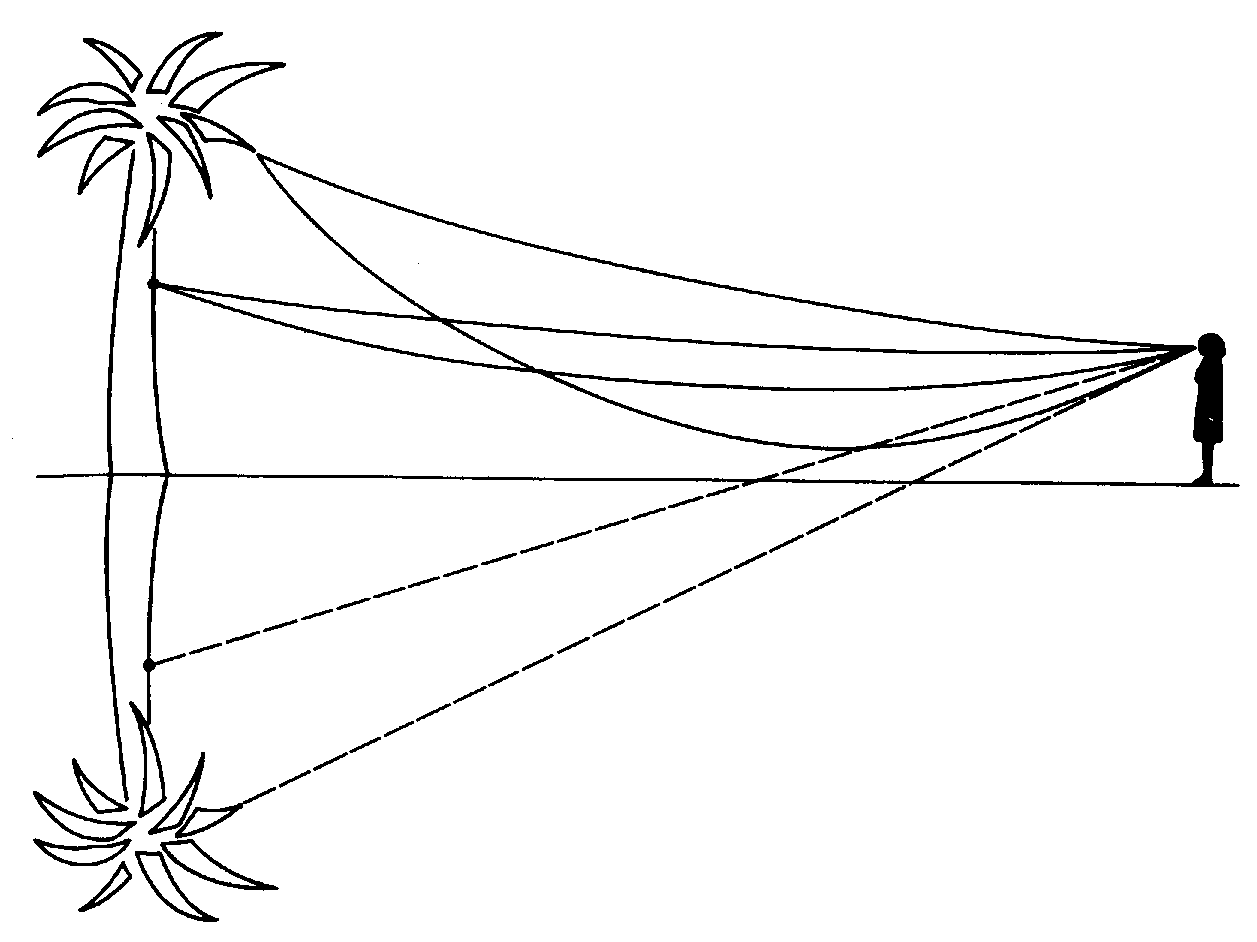
\includegraphics[width=0.4\textwidth]{./picture/FataEinleitung.png}
	\caption{Das Auge interpretiert, dass die Lichtstrahlen mit veränderter Richtung aus der tangentialen Verlängerung kommen und sieht dort das Bild}
	\label{Ab:fataEinleitung}
\end{figure}


\subsection{Untersuchung der Krümmungseigenschaften bei einer räumlichen Dichteänderung}

Bei einer Fata Morgana hat die Luft eine optische Dichte von $n(x,y)$. 
Dabei bewegt sich das Licht mit der Geschwindigkeit $c/n(x,y)$. 
Die benötigte Zeit, damit das Licht vom Punkt $(x_0, y_0)$ nach $(x_1, y_1)$ braucht,
kann mit dem Kurvenintegral berechnet werden.

\begin{equation}
T(y) = \int \limits_{x_0}^{x_1} \frac{n(x,y)}{c} \sqrt{1 + y'(x)^2} dx
\end{equation}

Wie es bei einem heissen Tag auf einer Strasse oder in einer Wüste zutrifft,
nehmen wir zuerst nur einmal an, dass die optische Dicht nur von $y$ abhängt
(also $n(x,y) = g(y)$) und mit zunehmenden $y$ ebenfalls zunimmt. 
Dies bedeutet für die Funktion $g(y)$, dass $g(y) > 0$ und $g'(y) > 0 $ ist.

Um dieses Minimalproblem zu lösen, wird die Euler-Lagrange-Gleichung des Variationsproblems aufgestellt (\eqref{krümmung}).

\begin{equation}
	T(y) = \int \limits_{x_0}^{x_1} \frac{g(y)}{c} \sqrt{1 + y'(x)^2} dx = \frac{1}{c} \int \limits_{x_0}^{x_1} g(y) \sqrt{1 + y'(x)^2} dx
	\label{krümmung}
\end{equation}

Der Faktor $\frac{1}{c}$ hat keinen Einfluss auf das Integral und somit auch nicht auf das Variationproblem, deshalb kann er weggelassen werden, um ihn nicht ständig mitschleppen zu müssen.
Es werden nun die Ableitungen der Funktion \ref{funktionRech} gebraucht. Sie sind in \ref{ableitungenLag} aufgeführt.
\begin{equation}
	F(x,y,y') = g(y) \sqrt{1 + y'^2}
	\label{funktionRech}
\end{equation}

\begin{align}
	\frac{\partial F}{\partial y} = g'(y) \sqrt{1 + y'^2} \notag \\
	\frac{\partial F}{\partial y'} = g(y) \frac{y'}{\sqrt{1 + y'^2}}
	\label{ableitungenLag}
\end{align}

Für die Euler-Lagrange-Gleichung muss man im zweiten Ausdruck für $y$ und $y'$, $y(x)$ 
und $y'(x)$ einsetzen und nach $\frac{d}{dx}$ ableiten, (\eqref{lagrange1}).

\begin{align}
	\frac{d}{dx} \frac{\partial F}{\partial y'} = \frac{d}{dx} (g(y(x)) \frac{y'(x)}{\sqrt{1 + y'(x)^2}})
	 = g'(y(x)) \frac{y'(x)^2}{\sqrt{1 + y'(x)^2}} + g(y(x)) \frac{y''(x)}{\sqrt{1 + y'(x)^2}} - \notag \\
	 g'(y(x)) \frac{y'(x)^2 y''(x)}{(1 + y'(x))^\frac{3}{2}} 
	 \label{lagrange1}
\end{align}

Auch im zweiten Term der Euler-Lagrange-Gleichung wird für $y'$ $y'(x)$ eingesetzt. Es ergibt sich \eqref{lagrange2}
\begin{align}
	0 = \frac{d}{dx} \frac{\partial F}{\partial y'} - \frac{\partial F}{\partial y} = 
	g'(y(x)) \frac{y'(x)^2}{\sqrt{1 + y'(x)^2}} + g(y(x)) \frac{y''(x)}{\sqrt{1 + y'(x)^2}} - \notag \\
	g'(y(x)) \frac{y'(x)^2 y''(x)}{(1 + y'(x)^2)^\frac{3}{2}}  - g'(y(x)) \sqrt{1 + y'(x)^2}
	\label{lagrange2}
\end{align}

Da $\sqrt{1 + y'(x)^2} > 0$ und somit nicht gleich Null ist kann die Gleichung mit $\sqrt{1 + y'(x)^2}$  multipliziert werden um einen einfacheren Ausdruck zu bekommen, (\eqref{lagrange3}).

\begin{align}
	0 = g'(y(x)) y'(x)^2 + g(y(x)) y''(x) - g'(y(x)) \frac{y'(x)^2 y''(x)}{(1 + y'(x)^2)} - \notag \\ 
	g'(y(x)) (1 + y'(x)^2)
	\label{lagrange3}
\end{align}

Auch $g(y(x))$ ist nicht gleich Null, da nach eingangs erfolgter Definition $g(y(x)) > 0$, eine Division mit $g(y(x))$ ist somit zulässig, (\eqref{lagrange4}).

\begin{align}
	\frac{g'(y(x))}{g(y(x))} (1 + y'(x)^2) - \frac{g'(y(x))}{g(y(x))} y'(x)^2 =  y''(x) - \frac{y'(x)^2 y''(x)}{(1 + y'(x)^2)} \notag \\
	\frac{g'(y(x))}{g(y(x))} (1 + y'(x)^2 - y'(x)^2) = \frac{\left(1 + y'(x)^2 \right)y''(x) - y'(x)^2 y''(x)}{(1 + y'(x)^2)} \notag \\
	\frac{g'(y(x))}{g(y(x))} = \frac{y''(x) + y'(x)^2 y''(x) - y'(x)^2 y''(x)}{(1 + y'(x)^2)} = \frac{y''(x)}{1 + y'(x)^2}
	\label{lagrange4}
\end{align}


\eqref{lagrange4} kann jetzt auf ihre Eigenschaften bezüglich der Krümmung untersucht werden. Gemäss den Definitionen von ganz am Anfang ist die linke Seite positiv. 
Der Nenner der rechte Seite ist ebenfalls positiv, daraus resultiert, dass der Zähler der rechten Seite ebenfalls positiv sein muss, (\eqref{krümmungAuswertung}).

\begin{align}
	\frac{g'(y(x))}{g(y(x))} > 0 \qquad \wedge \qquad (1 + y'(x)^2) > 0 \qquad \Rightarrow \qquad y''(x) > 0
	\label{krümmungAuswertung}
\end{align}

Da die zweite Ableitung positiv ist, muss die Funktion des Lichtstrahles konvex sein.
Dies bedeuted, dass der Lichtstrahl sich über dem Boden nach oben biegt, ganz egal wie die Funktion von $g(x)$ aussieht, solange sie monoton steigend ist.
Daraus kann die verallgemeinerte Schlussfolgerung gezogen werden, dass der Lichtstrahl konkav sein muss, wenn die Funktion $g(x)$ monoton fallend ist.
\begin{definition}
Ein Lichtstrahl wird in einem inhomogenen Medium in Richtung höherer Dichte gekrümmt, verhält sich die Dichteänderung monoton fallend oder steigend, nimmt der Lichtstrahl eine konvexe oder konkave Kurvenform an.
\index{Krümmung von Lichtstrahlen}
\end{definition}

\subsubsection{Technische Anwendung dieser Erkenntnis}
In einem Lichtwellenleiter wird dieses Phänomen ausgenutzt, indem die untere Seite des Lichtleiters eine monoton steigende
und die obere Seite des Lichtleiters eine monoton fallende Funktion ist. 
Dadurch ist dass Licht dann im Leiter ''gefangen'' und kann nicht über einen Rand hinausgehen.

\subsection{Berechnung der Differentialgleichung einer Fata Morgana}

eine änderung von x wird vernachlässigt da die Krümmung auf der Erdoberfläche vernachlässigbar ist
\begin{align}
\frac{n(x,y)}{c} \rightarrow \frac{g(y)}{c}
T(y) = \int \limits_{x_0}^{x_1} \frac{g(y)}{c} \cdot \textbf{ ??? } dx \notag \\
F(x,y,y') = g(y) \cdot \textbf{ ??? } \notag
\end{align}

Falls bei \textbf{???} nichts mehr kommt wäre die partielle Ableitung nach $y'$ = 0
\begin{align}
\frac{\partial F}{\partial y} = g'(y)\notag \\
\frac{\partial F}{\partial y'} = 0 \notag 
\end{align}
\begin{align}
g(y) \  und \ g'(y) \ durch \ y = m\cdot x + b \ und \ y' = m \ ersetzen \ \notag \\
\frac{d}{dx} \frac{\partial F}{\partial y'} = 0 \notag \\
	0 = \frac{d}{dx} \frac{\partial F}{\partial y'} - \frac{\partial F}{\partial y} = m
\end{align}

Was nicht sein kann.
Meine Frage:
muss ich bei \textbf{???} ebenfalls $\sqrt{1 + y'^2}$ für das Kurven Integral einsetzen da es sich um eine Krümmung handelt 
ich hätte dann
\begin{align}
	\frac{g'(y(x))}{g(y(x))} (1 + y'(x)^2) - \frac{g'(y(x))}{g(y(x))} y'(x)^2 =  y''(x) - \frac{y'(x)^2 y''(x)}{(1 + y'(x)^2)} \notag \\
	\frac{g'(y(x))}{g(y(x))} (1 + y'(x)^2 - y'(x)^2) = \frac{\left(1 + y'(x)^2 \right)y''(x) - y'(x)^2 y''(x)}{(1 + y'(x)^2)} \notag \\
	\frac{g'(y(x))}{g(y(x))} = \frac{y''(x) + y'(x)^2 y''(x) - y'(x)^2 y''(x)}{(1 + y'(x)^2)} = \frac{y''(x)}{1 + y'(x)^2} \notag
\end{align}
und würde in $y(x) = m\cdot x + b \ und \ y(x)' = m$

oder mache ich irgend etwas grundsätzlich falsch?


\subsection{Fata Morgana Spezifisch}

\begin{figure}[H]
	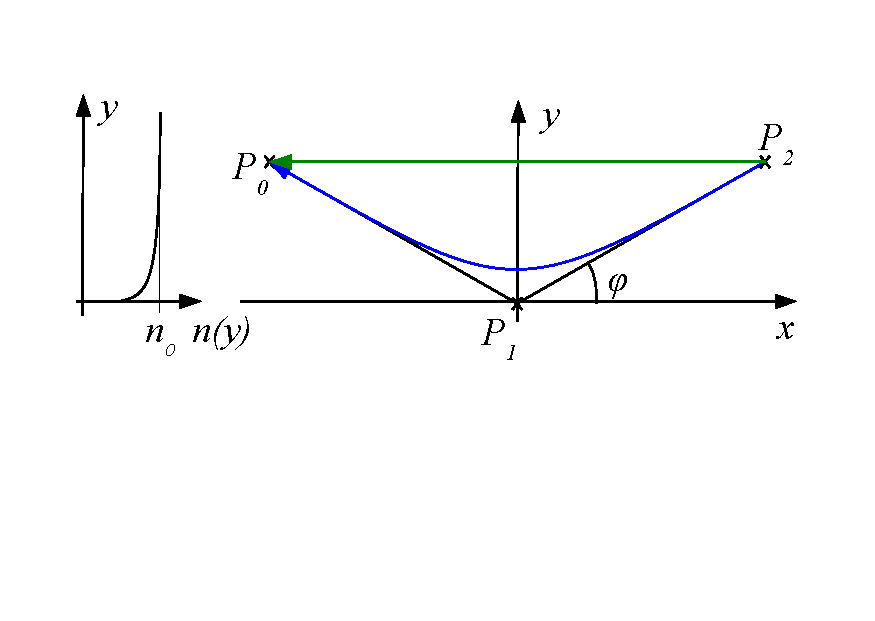
\includegraphics[width=0.8\textwidth]{./picture/FataMorgana.pdf}
	\caption{Skizze der Funktion einer Fata Morgana}
	\label{Ab:fata}
\end{figure}


Wir nehmen an, wir hätten eine Fata Morgana. 
Dabei hat der Brechungsindex die Funktion nach \eqref{brechungsindexFunktion} in Abhängigkeit von $y$ 
(Der Höhe über dem Boden).

\begin{equation}
	n = n_0 (1 - \varepsilon e^{- \alpha y})
	\label{brechungsindexFunktion}
\end{equation}

\texttodo{welcher effekt ist relativ klein?}
Dabei ist der Effekt relativ klein, da $\epsilon << 1$ ist und 
die Skalenlänge $\alpha$ in der Grössenordnung von $\alpha = 1 \cdot m^{-1}$ ist.
Zusätzlich können wir für die Skalierung der x-Richtung die nach \eqref{lichtge} definierte konstante $C$ einführen.

\begin{equation}
	C = n \frac{dx}{ds}
	\label{lichtge}
\end{equation}

Wenn die Strahlengleichung komponentenweise für $r = (y(x), x)$ betrachten wird kann daraus die Strahlengleichung, \eqref{strahlengleichung}, hergeleitet werden.

\begin{equation}
\frac{d}{ds} \left ( n \frac{dy}{ds} \right ) = \frac{d}{dx} \left ( n \frac{dy}{dx} \frac{dx}{ds} \right ) \frac{dx}{ds} =
\frac{d}{dx} \left ( C \frac{dy}{dx} \right ) \frac{C}{n} = \frac{\partial n(y)}{\partial y}
\label{strahlengleichung}
\end{equation}

Da die Konstante $C$ nur die x-Achse skaliert, wird diese auf den Wert $1$ festgelegt.
Wegen 
\texttodo{stimmt diese gleichung? $2 n \partial n / \partial y = \partial n^2 / \partial y$ meiner meinung nach geht da faktor 2 verloren, ist aber schon spät in der Nacht}
\begin{equation}
	2 n \partial n / \partial y = \partial n^2 / \partial y \qquad \text{und} \qquad n^2 \simeq n_0^2(1 - 2 \varepsilon e^{-\alpha y}) \notag
\end{equation}erhalten wir \eqref{difGleich}.

\begin{equation}
	\frac{d^2 y(x)}{dx^2} = \frac{1}{2} \frac{\partial}{\partial y} n^2(y) = n_0^2 \varepsilon \alpha e^{-\alpha y}
	\label{difGleich}
\end{equation}

Diese Gleichung kann mit elementaren Methoden gelöst werden. 
Zudem wird der Steigungswinkel $\varphi$ eingeführt daraus ergibt sich
$\kappa = (\frac{\alpha}{2}) \tan(\varphi)$ daraus ergibt sich die übersichtlichere \eqref{fataFunktion}.
\texttodo{verständlich beschreiben mit zwischen schritten damit sich die diffgleichung und die funktion die gefunden wird ersichtlich sind}
\begin{equation}
	y = y_0 + \frac{1}{\alpha} ln(\cosh^2(\kappa(x - x_0))) \xrightarrow{\kappa (x - x_0 ) >> 1} y =	y_0 + \frac{2 \kappa}{\alpha} (x - x_0)
	\label{fataFunktion}
\end{equation}


In grossen Abständen zum Spiegelpunkt $x_0$ ist die Ausbreitung des Lichtes geradlinig.
Der Beobachter sieht, wie erwarted zwei Bilder, wobei eines auf dem Kopf steht.

\subsection{Lichtwellenleiter}

Hier kommt das vierte Beispiel.